% main.tex  --- IEEEtran + TikZ 完全版
\documentclass[conference]{IEEEtran}

% ---------- Packages ----------
\usepackage{amsmath,amssymb}
\usepackage{graphicx}
\usepackage{booktabs}
\usepackage{siunitx}
\usepackage{hyperref}
\usepackage{placeins} % \FloatBarrier
\usepackage{tikz}
\usetikzlibrary{arrows.meta,positioning,shapes,fit}

% ---------- TikZ styles ----------
\tikzset{
  box/.style   = {draw, rounded corners=2pt, minimum width=2.6cm, minimum height=8mm, align=center},
  pale/.style  = {fill=gray!10},
  line/.style  = {-{Latex[length=2mm]}, thick},
}

% ---------- Title ----------
\title{AITL on Space: A Robust Three-Layer Architecture\\
with a Tri-NVM Hierarchy (SRAM / MRAM / FRAM)\\
for Long-Duration Spacecraft Autonomy}

\author{%
  \IEEEauthorblockN{Shinichi Samizo}
  \IEEEauthorblockA{Independent Semiconductor Researcher\\
Former Engineer at Seiko Epson Corporation\\
Email: shin3t72@gmail.com \quad GitHub: \url{https://github.com/Samizo-AITL}}
}

\begin{document}
\maketitle

\begin{abstract}
We propose AITL on Space, a three-layer control architecture (Robust Core, FSM Supervisor, AI Adaptor) implemented on a \SI{22}{nm} FD\!SOI SoC with a hardened Tri-NVM hierarchy (SRAM/MRAM/FRAM). The system targets ultra-robust autonomy under radiation, thermal cycling, and long-term drift. This paper outlines the architecture, an 11D state-space plant model (8--20D extensible), an $H_\infty$ mixed-sensitivity design flow, and a verification pipeline from FPGA HIL to ASIC.
\end{abstract}

\IEEEpeerreviewmaketitle

% ===== Fig.1: Architecture (2段幅、Abstractの後、上部固定) =====
\begin{figure*}[t]
  \centering
  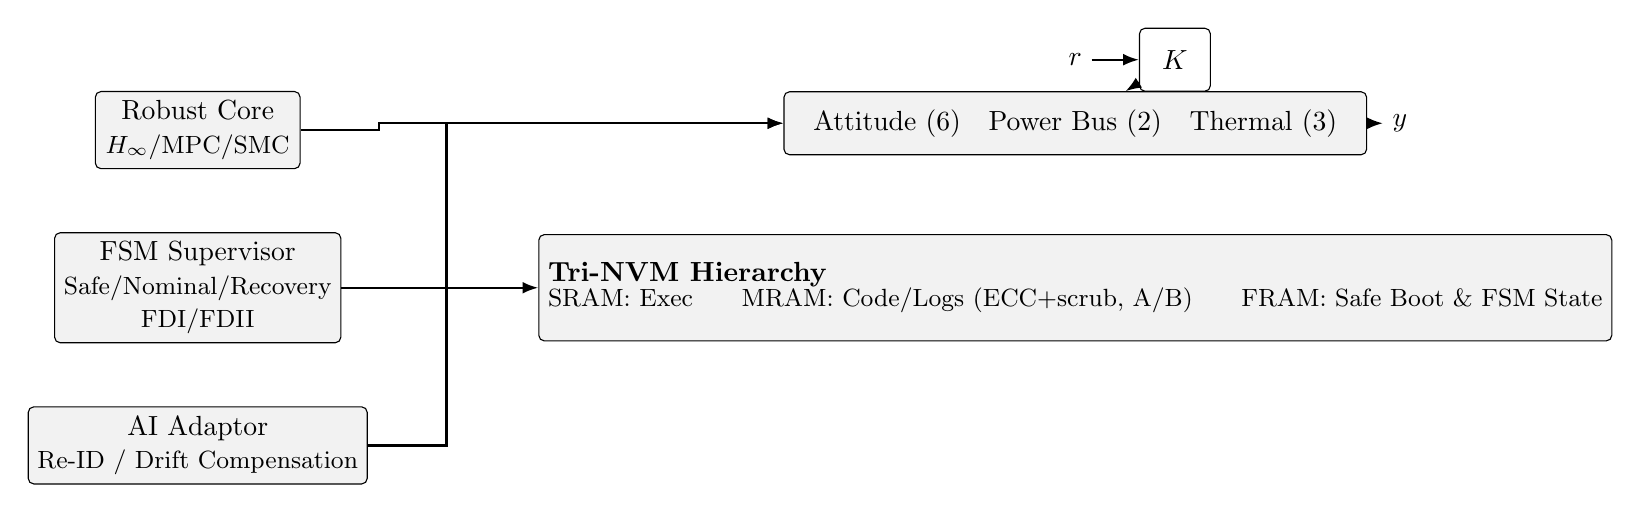
\begin{tikzpicture}[node distance=8mm]
    % Left column (three layers)
    \node[box,pale] (robust) {Robust Core\\ \small $H_\infty$/MPC/SMC};
    \node[box,below=of robust,pale] (fsm) {FSM Supervisor\\ \small Safe/Nominal/Recovery\\ \small FDI/FDII};
    \node[box,below=of fsm,pale] (ai) {AI Adaptor\\ \small Re-ID / Drift Compensation};

    % Plant and tri-NVM (center/right)
    \node[box, right=25mm of fsm, minimum width=7.4cm, minimum height=1.35cm, pale, align=left] (nvm) {%
      \textbf{Tri-NVM Hierarchy}\\[-1mm]
      \small SRAM: Exec \hspace{4mm}
      MRAM: Code/Logs (ECC{+}scrub, A/B) \hspace{4mm}
      FRAM: Safe Boot \& FSM State};

    \node[box, above=10mm of nvm, minimum width=7.4cm, pale] (plant) {Attitude (6)\quad Power Bus (2)\quad Thermal (3)};

    % Wires from layers to NVM/Plant
    \draw[line] (robust.east) -- ++(10mm,0) |- (plant.west);
    \draw[line] (fsm.east) -- ++(10mm,0) |- (nvm.west);
    \draw[line] (ai.east) -- ++(10mm,0) |- (plant.west);

    % Plant I/O
    \node[above=2mm of plant] (r) {$r$};
    \node[right=2mm of plant] (y) {$y$};
    \node[box,minimum width=0.9cm,minimum height=0.8cm, right=6mm of r] (K) {$K$};
    \draw[line] (r) -- (K);
    \draw[line] (K) -- (plant);

    \draw[line] (plant) -- (y);

    % Labels
    \node[below=1.0cm of nvm] (dummy) {};
  \end{tikzpicture}
  \caption{AITL on Space architecture with Robust Core, Supervisor FSM, AI Adaptor, and the Tri-NVM hierarchy.}
  \label{fig:arch}
\end{figure*}

\FloatBarrier % ← Abstract直後の配置をここで固定

% ===== Body =====
\section{Introduction}
Long-duration missions require high availability under TID/SEE and thermal cycles. Conventional PID{+}Flash architectures face reliability limits. We summarize related work and motivate AITL on Space.

\section{System Architecture}
AITL comprises: (i) Robust Core (for $H_\infty$/MPC/SMC), (ii) FSM Supervisor (Safe/Nominal/Recovery, FDI/FDII), and (iii) AI Adaptor for long-term re-identification. A Tri-NVM hierarchy---SRAM for execution, MRAM for logs/code (ECC{+}scrub, A/B slots), and FRAM for safe boot---ensures persistence.

% ===== Fig.2: Hinf closed-loop (1段幅) =====
\begin{figure}[t]
  \centering
  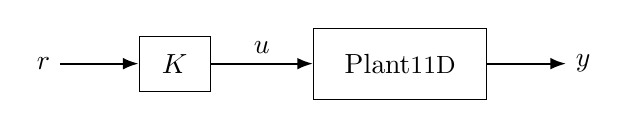
\begin{tikzpicture}
    \node[draw,minimum width=0.9cm,minimum height=0.7cm] (K) {$K$};
    \node[draw,minimum width=2.2cm,minimum height=0.9cm, right=13mm of K] (P) {Plant\\ \small 11D};
    \node[left=10mm of K] (r) {$r$};
    \node[right=10mm of P] (y) {$y$};
    \draw[line] (r) -- (K);
    \draw[line] (K) -- node[above] {$u$} (P);
    \draw[line] (P) -- (y);
  \end{tikzpicture}
  \caption{Closed-loop schematic used for $H_\infty$ synthesis on the 11D plant.}
  \label{fig:closedloop}
\end{figure}

\section{Mathematical Model}
We use an 11D discrete-time plant that couples attitude (6), power bus (2), and thermal nodes (3):
\begin{align}
  x_{k+1} &= A x_k + B u_k + E w_k,\\
  y_k &= C x_k + D u_k + v_k .
\end{align}
Extensions scale to 20D with translational axes and bias states.

\section{$H_\infty$ Mixed-Sensitivity Design}
Weights $(W_1,W_2,W_3)$ shape sensitivity, effort, and complementary sensitivity. \textit{EduController} exports JSON plant/weights; \textit{AITL-H} synthesizes output-feedback $K$ and fixed-point realization.

\section{Verification Pipeline}
FPGA HIL injects SEU bursts and sensor outages; metrics include safe-mode time ($<\SI{1}{s}$), recovery rate ($\ge\! \SI{99}{\%}$), and ECC statistics. Physical design proceeds to 22FDX tape-out; SystemDK FEM closes thermal/packaging effects.

% ===== Fig.3: Verification flow (1段幅) =====
\begin{figure}[t]
  \centering
  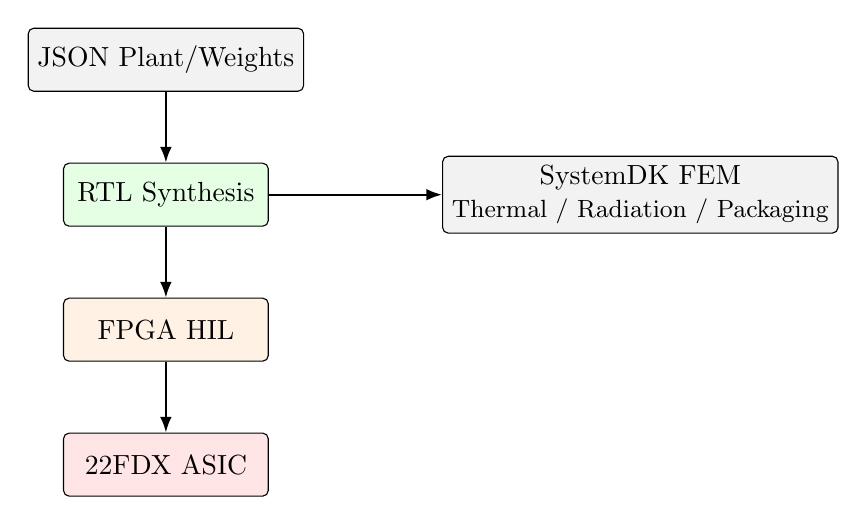
\begin{tikzpicture}[node distance=9mm]
    \node[box,pale] (json) {JSON Plant/Weights};
    \node[box,pale,below=of json,fill=green!10] (rtl) {RTL Synthesis};
    \node[box,pale,below=of rtl,fill=orange!10] (hil) {FPGA HIL};
    \node[box,pale,below=of hil,fill=red!10] (asic) {22FDX ASIC};
    \node[box,pale,minimum width=4.5cm, right=22mm of rtl] (fem) {SystemDK FEM\\ \small Thermal / Radiation / Packaging};

    \draw[line] (json) -- (rtl);
    \draw[line] (rtl) -- (hil);
    \draw[line] (hil) -- (asic);
    \draw[line] (rtl) -- (fem);
  \end{tikzpicture}
  \caption{Verification pipeline from JSON design to RTL, FPGA HIL, and ASIC; FEM closes the loop with thermal and radiation scenarios.}
  \label{fig:pipeline}
\end{figure}

\FloatBarrier

\section{Conclusion}
AITL on Space offers a practical path to resilient autonomy for deep-space missions.

% ---------- References ----------
\begin{thebibliography}{99}
\bibitem{doyle} G.~Doyle, \textit{Feedback Control Theory}.
\bibitem{colinge} J.-P.~Colinge, \textit{Silicon-on-Insulator Technology}.
\end{thebibliography}

% ---------- Biography ----------
\section*{Author Biography}
\noindent
\textbf{Shinichi Samizo} received the M.S. degree in Electrical and Electronic Engineering from Shinshu University, Japan. He worked at Seiko Epson Corporation as an engineer in semiconductor memory and mixed-signal device development, and contributed to inkjet MEMS actuators and PrecisionCore printhead technology. He is currently an independent semiconductor researcher focusing on process/device education, memory architecture, and AI system integration. Contact: \texttt{shin3t72@gmail.com}.

\end{document}
